\documentclass[pdftex,letterpaper,12pt]{report}
\usepackage{thesis}
\usepackage{amsmath}
\usepackage{amssymb}
\usepackage{amsthm}
\usepackage{mathtools}
\usepackage{bm}
\usepackage{gensymb}
\usepackage{wasysym}
\usepackage{mathtools}
\usepackage{physics}
\usepackage{empheq}
\usepackage{cases}
\usepackage{rotating}
\usepackage{subfig}
\usepackage{caption}
\usepackage{multirow}
\captionsetup{labelfont=bf} 
\captionsetup[subfloat]{position=top,singlelinecheck=off,justification=raggedright,font=bf,labelfont=large,labelformat=simple,captionskip=-2mm}
\usepackage{float}
\usepackage{enumitem} 
\usepackage[toc,page]{appendix}






\begin{document}
	
\begin{subequations}\label{InitialSpinup}
	\begin{gather}
	P_{pc}(t)=\gamma_{se}P_{A}t-\frac{1}{2}\gamma_{se}P_{A}(\gamma_{se}+\Gamma_{pc}+d_{pc})t^{2}\\
	P_{tc}(t)=\frac{1}{2}\gamma_{se}P_{A}d_{tc}t^{2}
	\end{gather}
\end{subequations}

\begin{equation}
\langle \gamma_{se}\rangle=\frac{\Gamma_{s}-\langle \Gamma\rangle+\delta\Gamma}{1+X}
\end{equation}

$(\Gamma_{s}-\langle \Gamma\rangle)$  

\begin{table*}\tiny
	\captionsetup{font=scriptsize}
	\begin{center}
		\def\arraystretch{0.75}
		\setlength\tabcolsep{0.5pt}
		\begin{tabular}{|c|c|ccc|ccc|ccccc|cc|c|}
			\hline
			\multirow{2}{*}{\begin{sideways}{EXP}\end{sideways}}&\multirow{2}{*}{Cell} & \multirow{2}{*}{Lasers} & $I_0$ & T$_\mathrm{pc}^\mathrm{set}$ & \multirow{2}{*}{$P_\mathrm{He}^\infty$} & $\Gamma_\mathrm{s}^{-1}$ & $\langle\Gamma\rangle^{-1}$ & \multirow{2}{*}{$\langle P^\mathrm{A} \rangle$} & \multirow{2}{*}{$P_\mathrm{line}^\mathrm{A}$} & \multirow{2}{*}{$D_\mathrm{fr}$} & \multirow{2}{*}{$D_\mathrm{pb}$} & [Rb]$_\mathrm{fr}$ & $\Delta$T$_\mathrm{Rb}$ & $\Delta$T$_\mathrm{He}$ & \multirow{2}{*}{X}\\
			&& & W/cm$^2$ & $^\circ$C & & hrs & hrs & & & & & $10^{14}$/cm$^3$ & $^\circ$C & $^\circ$C &\\
			\hline
			\hline
			\multirow{5}{*}{\begin{sideways}saGDH\end{sideways}} & Proteus & 3B & 3.8 & 180 & 0.46 & 27 & 74 & - & - & 0 & 0 & - & - & - & -\\
			\cline{2-16}
			& Priapus & 3B & 3.8 & 180 & 0.44 & 21 & 56 & - & - & 0 & 0 & - & - & - & -\\
			\cline{2-16}
			& Penelope & 3B & 3.8 & 180 & 0.39 & 18 & 46 & - & - & 0 & 0 & - & - & - & -\\
			\cline{2-16}
			& Powell & 3B & 3.8 & 180 & 0.38 & 13 & 25 & - & - & 0 & 0 & - & - & - & -\\
			\cline{2-16}
			& Prasch & 3B & 3.8 & 180 & 0.33 & 13 & 33 & - & - & 0 & 0 & - & - & - & -\\
			\hline
			\hline
			\multirow{20}{*}{\begin{sideways}GEN\end{sideways}} & \multirow{2}{*}{Al} & 2.5B & 3.2 & 235 & 0.53(03) & 7.86(05) & 27.42(1.37) & - & - & - & 4.53(25) & - & - & - & - \\
			& & 5B & 6.1 & 235 & 0.54(03) & 6.73(18) & 27.42(1.37) & - & - & - & 4.53(25) & - & - & - & - \\
			\cline{2-16}
			& \multirow{2}{*}{Barbara} & 2.5B & 1.6 & 235 & 0.37(02) & 5.5(08) & 42.95(2.15) & - & - & - & 4.80(25) & - & - & - & - \\
			& & 5B & 3.1 & 235 & 0.57(03) & 4.76(63) & 42.95(2.15) & - & - & - & 4.80(25) & - & - & - & - \\
			\cline{2-16}
			& Gloria & 3B & 1.7 & 235 & 0.60(03) & 6.13(04) & 38.29(1.91) & - & - & - & 7.20(40) & - & - & - & - \\
			\cline{2-16}
			& \multirow{2}{*}{Anna} & 1B & 0.6 & 235 & 0.33(02) & 5.60(34) & 11.38(57) & - & - & - & 9.64(57) & - & - & - & - \\
			& & 1.5B & 1.0 & 235 & 0.39(02) & 5.37(08) & 11.38(57) & - & - & - & 9.64(57) & - & - & - & - \\
			\cline{2-16}
			& \multirow{2}{*}{Dexter} & 1.5B & 1.5 & 235 & 0.47(02) & 7.58(17) & 18.45(92) & - & - & - & - & - & - & - & - \\
			& & 5B & 6.1 & 235 & 0.49(02) & 6.63(12) & 18.45(92) & - & - & - & - & - & - & - & - \\
			\cline{2-16}
			& Edna & 3B & 2.4 & 235 & 0.56(03) & 5.71(02) & 27.42(1.37) & - & - & - & 3.63(20) & - & - & - & - \\
			\cline{2-16}
			& \multirow{2}{*}{Dolly} & 3B & 1.0 & 235 & 0.43(02) & 6.16(03) & 35.24(1.76) & - & - & - & 20(1.3) & - & - & - & - \\
			& & 1N1B & 1.4 & 235 & 0.62(03) & 5.79(07) & 35.24(1.76) & - & - & - & 20(1.3) & - & - & 17(10) & - \\
			\cline{2-16}
			& \multirow{3}{*}{Simone} & 2N1B & 3.8 & 215 & 0.31(01) & 14.08(06) & 22.87(1.14) & 0.947(020)  & 0.91(05) & 10.66(54) & 8.89(45) & 0.20(02) & -7(3) & - & -0.04(12)$^\star$ \\
			& & 2N1B & 3.8 & 240 & 0.48(02) & 6.89(20) & 22.87(1.14) & - & - & - & 9.76(49) & - & - & - & - \\
			& & 2N1B & 3.8 & 255 & 0.58(02) & 6.45(10) & 22.98(1.14) & 0.929(023) & 0.92(05) & 12.48(83) & 10.3(52) & 0.90(09) & -4(5) & - & 0.11(06)$^\star$ \\
			\cline{2-16}
			& \multirow{5}{*}{Sosa} & 2N1B & 1.9 & 160 & 0.57(02) & 16.69(09) & 73.68(3.68) & 0.966(020) & 1.00(03) & 0 & 0 & 1.97(13) & 4(1) & 30(7) & 0.24(06)$^\dagger$ \\
			&  & 2N1B & 1.9 & 170 & 0.61(03) & 11.67(04) & 73.68(3.68) & 0.964(020) & 0.98(03) & 0 & 0 & 3.00(33) & 3(3) & 38(14) & 0.27(06)$^\star$ \\
			&  & 2N1B & 1.9 & 180 & 0.55(02) & 8.79(09) & 73.68(3.68) & 0.954(022) & 0.97(03) & 0 & 0 & 4.30(27) & 1(2) & 47(7) & 0.43(06)$^\dagger$ \\
			&  & 2N1B & 1.9 & 190 & 0.40(02) & 6.39(22) & 73.68(3.68) & 0.854(075) & 0.82(03) & 0 & 0 & 5.69(63) & -2(3) & 48(20) & 0.58(12)$^\star$ \\
			&  & 2N1B & 1.9 & 200 & 0.26(01) & 5.04(17) & 73.68(3.68) & - & - & 0 & 0 & - & - & 43(18) & - \\
			%& 2C1F & 1.9 & 160 & 0.57(03) & 16.7(09) & 55.7(1.8) & 1.00(03) & 0 & 0 & -\\
			% & 2C1F & 1.9 & 170 & 0.61(03) & 11.7(03) & 55.5(2.0) & 0.98(03) & 0 & 0 & -\\
			% & 2C1F & 1.9 & 180 & 0.55(03) & 8.79(09) & 55.2(2.2) & 0.97(03) & 0 & 0 & - \\
			% & 2C1F & 1.9 & 190 & 0.40(02) & 6.39(22) & 55.1(2.3) & - & 0 & 0 & -\\
			% & 2C1F & 1.9 & 200 & 0.26(01) & 5.40(17) & 55.4(2.1) & 0.83(17) & 0 & 0 & -\\
			\hline
			\hline
			\multirow{12}{*}{\begin{sideways}Transversity\end{sideways}} & Boris & 3B & 1.8 & 235 & 0.42(02) & 6.25(04) & 23.74(1.19) & 0.871(050) & 0.79(07) & 1.96(18) & 2.45(23) & 2.19(34) & -8(7) & - & 0.26(10)$^\star$ \\
			\cline{2-16}
			& \multirow{2}{*}{Samantha} & 3B & 1.8 & 235 & 0.50(02) & 6.30(13) & 36.51(1.83) & - & - & - & 4.34(23) & - & - & - & -\\
			& & 3N & 2.6 & 235 & 0.68(03) & 4.62(03) & 22.13(1.11) & 0.956(020) & 0.99(03) & 4.37(10) & 4.34(23) & 1.80(10) & 7(2) & 21(10) & 0.12(05)$^\star$\\
			\cline{2-16}
			& Alex & 2N1B & 2.6 & 235 & 0.59(03) & 4.81(02) & 32.96(1.65) & 0.942(042) & 0.99(03) & 1.37(08) & 1.19(07) & 4.08(36) & 0(4) & 42(10) & 0.34(06)$^\dagger$ \\
			\cline{2-16}
			& Moss & 1N1B & 1.8 & 235 & 0.62(03) & 5.35(04) & 33.00(1.65) & - & 0.95(09) & - & 2.40(13) & - & - & 29(8) & -\\
			\cline{2-16}
			& Tigger & 1N1B & 1.8 & 235 & 0.51(02) & 4.89(05) & 12.62(63) & - & 0.95(09) & - & - & - & - & 23(9) & -\\
			\cline{2-16}
			& Astral & 2N1B & 2.6 & 235 & 0.69(03) & 6.57(12) & 48.90(2.45) & 0.954(020) & 0.99(03) & 7.09(55) & 6.21(56) & 0.97(09) & 3(5) & 25(4) & 0.17(05)$^\dagger$\\
			\cline{2-16}
			& Stephanie & 3N & 2.6 & 235 & 0.63(03) & 4.55(09) & 48.35(2.42) & 0.929(114) & 0.99(03) & 1.39(11) & 1.50(10) & 5.08(58) & 7(5) & 54(6) & 0.31(08)$^\star$\\
			\cline{2-16}
			& \multirow{3}{*}{Brady} & 1N & 0.9 & 235 & 0.62(03) & 4.82(1.08) & 33.50(1.68) & - & 0.95(03) & - & 2.36(24) & -  & - & 14(9) & -\\
			& & 2N & 1.8 & 235 & 0.68(03) & 5.52(70) & 33.50(1.68) & - & 0.99(03) & - & 2.36(24) & - & - & 25(8) & -\\
			& & 3N & 2.6 & 235 & 0.70(03) & 5.30(01) & 33.50(1.68) & 0.956(021) & 0.99(03) & 2.60(20) & 2.36(24) & 2.86(30) & 6(5) & 39(9) & 0.14(05)$^\dagger$\\
			\cline{2-16}
			& Maureen & 3N & 2.6 & 235 & 0.66(03) & 5.42(12) & 29.21(1.46) & - & 0.97(09) & - & 4.42(55) & - & - & 32(12) & -\\
			\cline{2-16}
			&Antoinette & 3N & 1.7 & 215 & 0.49(02) & 6.63(37) & 20.93(1.05) & 0.958(020) & 0.99(03) & 2.85(13) & - & 0.96(07) & 0(3) & 16(8) & 0.28(08)$^\dagger$\\
			& & 3N & 1.7 & 235 & 0.61(03) & 4.18(10) & 20.93(1.05) & 0.936(043) & 0.99(03) & 3.32(27) & - & 1.83(20) & 0(5) & 20(10) & 0.24(07)$^\dagger$\\
			& & 3N & 1.7 & 255 & 0.41(02) & 2.66(11) & 20.93(1.05) & 0.776(099) & 0.93(10) & 3.57(23) & - & 2.88(39) & -5(6) & 33(9) & 0.55(13)$^\dagger$\\
			\hline
		\end{tabular}
		\caption
		{Cell Performance for three sets of experiments: saGDH (top), GEN (middle), and Transversity \& $d_2^n$ (bottom).  Within each experiment grouping, data is grouped by type of laser used (B = Broadband, N = Narrowband). $I_0$ is the nominal incident laser intensity at the center of the pumping chamber. $T_{pc}^{set}$ is the oven set temperature. $P_{pc}^\infty$ is the equilibrium polarization in the pumping chamber and $\Gamma_s$ is the slow time constant extracted from the five parameter fit to the polarization build up curve. $\Gamma_c$ is the cell-averaged room temperature spin relaxation rate. $\langle P_A\rangle/P_A^l$ is the volume averaged to line averaged alkali polarizaiton ratio determined from the optical pumping simulation. $P_A^l$ is the measured line averaged alkali polarization. $D_{fr} \& D_{pb}$ are the K to Rb density ratios determined from Faraday rotation and pressure broadening measurements. [Rb]$_{fr}$ is the Rb number density measured from Faraday rotation. $\Delta T_{He}$ is the temperature of Rb inferred from the number density relative to the oven set temperature. $\Delta T_{He}$ is the temperature of $^3$He inferred from temperature tests relative to the oven set temperature. X is the best combined value for the X-factor. $^\star$ indicates X was measured using only spinup, alkali polarization, and Faraday rotation data. $^\dagger$ indicates X was also measured using the early-time behavior of the spinup.}
	\end{center}
	\label{table:CellTable}
\end{table*}

The coefficients of pressure broadening for $^{3}$He, $^{4}$He and N$_{2}$ are listed in Table~\ref{PBCoef}.

\begin{figure}[H]
	\label{spinup}
	\centering
	\resizebox{0.91\textwidth}{!}{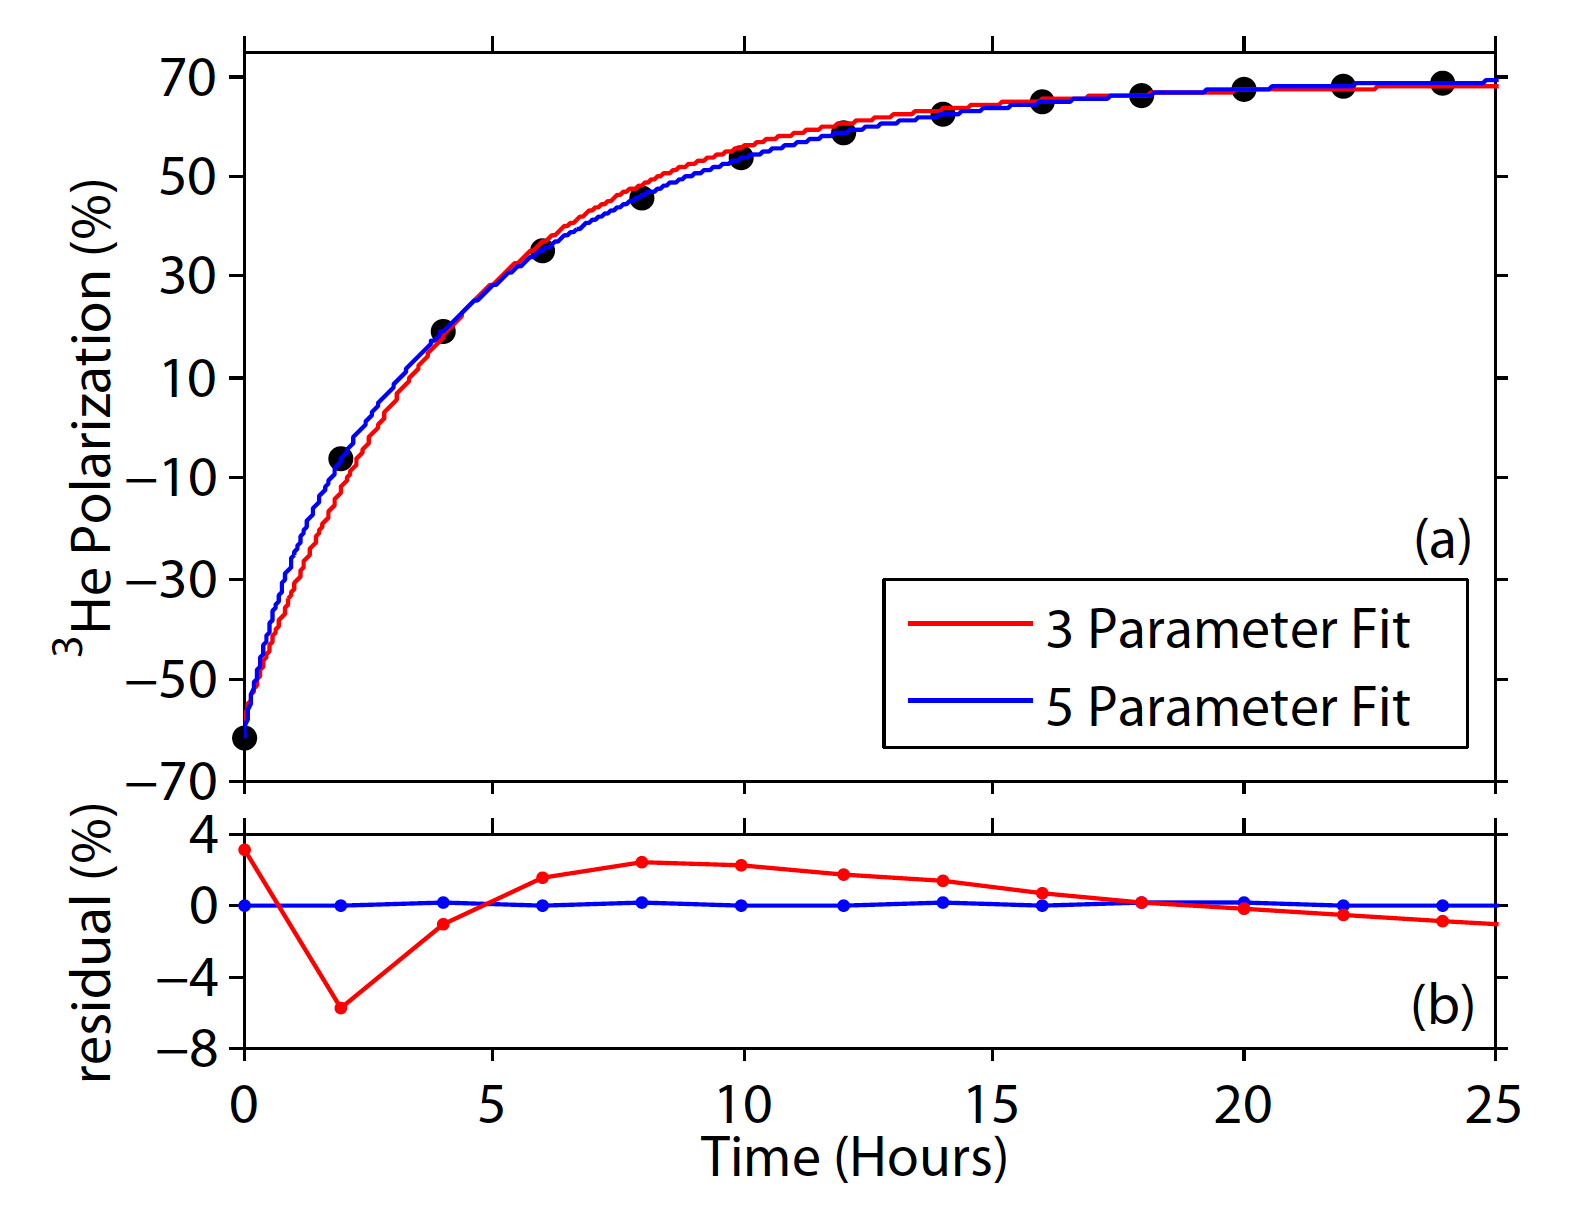
\includegraphics{Spinup.png}}
	\caption{{(a) Shown is a spinup of the target Brady. The spinup data has been fit with a 3-parameter and a 5-parameter formalism. (b) The residuals of the two fits. The error for 3-parameter fit is larger because it does not account for diffusion between two chambers. Adopted from~\cite{PhysRevC.91.055205}.}}
\end{figure}
	
The energy levels of $^{87}$Rb are shown in Fig.~\ref{fig:foms}.
where $\Gamma_{A}$ is the pressure dependent FWHM, $\Gamma_{A}\approx 0.04nm/amg \cdot [^{3}He]$.

\addcontentsline{toc}{chapter}{Bibliography}
\bibliography{ref}

\end{document}